% !TeX root = forth.tex
% !TeX spelling = en_US

\annex{Rationale} % A. (informative annex)}}}
\label{annex:rationale}
\setwordlist{core}

\ifinline\else
	\namespace{rat}
	\defersection{}
\fi

\newcommand{\readrationale}[1]{%
	\ifinline
		\begin{editor}
			In the \emph{review} (r) version of the document the
			rationale text for each of the words is given in with
			the main definition of the word.  The rationale for
			words in the \textbf{#1} word set will appear here in
			the final document.
		\end{editor}
	\else
		\defersection{}
		\input{r-#1.sub}
		\stepsection
	\fi
}

\section{Introduction} % A.1

\subsection{Purpose} % A.1.1

\subsection{Scope} % A.1.2
\label{rat:scope}

When judging relative merits of proposed changes to the standard, the
members of the committee were guided by the following goals (listed
in alphabetic order):

\begin{tabular}{lp{0.75\textwidth}}
Consistency	&
	The standard provides a functionally complete set of words with
	minimal functional overlap.
	\\[\parskip]
Cost of compliance &
	This goal includes such issues as common practice, how much
	existing code would be broken by the proposed change, and the
	amount of effort required to bring existing applications and
	systems into conformity with the standard.
	\\[\parskip]
Efficiency &
	Execution speed, memory compactness.
	\\[\parskip]
Portability	&
	Words chosen for inclusion should be free of system-dependent
	features.
	\\[\parskip]
Readability &
	Forth definition names should clearly delineate their behavior.
	That behavior should have an apparent simplicity which supports
	rapid understanding. Forth should be easily taught and support
	readily maintained code.
	\\[\parskip]
Utility	&
	Be judged to have sufficiently essential functionality and
	frequency of use to be deemed suitable for inclusion.
\end{tabular}


\section{Terms and notation} % A.2

\subsection{Definitions of terms} % A.2.1

\begin{description}
\item[aligned]~

Data can only be loaded from and stored to addresses that are aligned
according to the alignment requirements of the accessed type.  Field
offsets that are added to structure addresses also need to be aligned.

\item[ambiguous condition] ~

The response of a Standard System to an ambiguous condition is left
to the discretion of the implementor. A Standard System need not
explicitly detect or report the occurrence of ambiguous conditions.

\item[cross compiler] ~

Cross compilers may be used to prepare a program for execution in an
embedded system, or may be used to generate Forth kernels either for
the same or a different run-time environment.

\item[data field] ~

In earlier standards, data fields were known as ``parameter fields''.

On subroutine threaded Forth systems, everything is object code.
There are no traditional code or data fields. Only a word defined by
\word{CREATE} or by a word that calls \word{CREATE} has a data field.
Only a data field defined via \word{CREATE} can be manipulated portably.

\item[word set] ~

This standard recognizes that some functions, while useful in certain
application areas, are not sufficiently general to justify requiring
them in all Forth systems. Further, it is helpful to group Forth
words according to related functions. These issues are dealt with
using the concept of word sets.

The ``Core'' word set contains the essential body of words in a Forth
system. It is the only ``required'' word set. Other word sets defined
in this standard are optional additions to make it possible to
provide Standard Systems with tailored levels of functionality.
\end{description}

\subsection{Notation} % A.2.2

\addtocounter{subsubsection}{1}
\subsubsection{Stack notation} % A.2.2.2

The use of \emph{-sys}, \emph{orig}, and \emph{dest} data types in
stack effect diagrams conveys two pieces of information. First, it
warns the reader that many implementations use the data stack in
unspecified ways for those purposes, so that items underneath on
either the control-flow or data stacks are unavailable. Second, in
cases where \emph{orig} and \emph{dest} are used, explicit pairing
rules are documented on the assumption that all systems will
implement that model so that its results are equivalent to employment
of some stack, and that in fact many implementations do use the data
stack for this purpose. However, nothing in this standard requires
that implementations actually employ the data stack (or any other)
for this purpose so long as the implied behavior of the model is
maintained.


\section{Usage requirements} % A.3

Forth systems are unusually simple to develop, in comparison with
compilers for more conventional languages such as C. In addition to
Forth systems supported by vendors, public-domain implementations and
implementation guides have been widely available for nearly twenty
years, and a large number of individuals have developed their own
Forth systems. As a result, a variety of implementation approaches
have developed, each optimized for a particular platform or target
market.

The committee has endeavored to accommodate this diversity by
constraining implementors as little as possible, consistent with a
goal of defining a standard interface between an underlying Forth
System and an application program being developed on it.

Similarly, we will not undertake in this section to tell you how to
implement a Forth System, but rather will provide some guidance as
to what the minimum requirements are for systems that can properly
claim compliance with this standard.

\subsection{Data types} % A.3.1
\label{rat:types}

Most computers deal with arbitrary bit patterns. There is no way to
determine by inspection whether a cell contains an address or an
unsigned integer. The only meaning a datum possesses is the meaning
assigned by an application.

When data are operated upon, the meaning of the result depends on
the meaning assigned to the input values. Some combinations of input
values produce meaningless results: for instance, what meaning can
be assigned to the arithmetic sum of the ASCII representation of the
character ``A'' and a TRUE flag? The answer may be ``no meaning'';
or alternatively, that operation might be the first step in
producing a checksum. Context is the determiner.

The discipline of circumscribing meaning which a program may assign
to various combinations of bit patterns is sometimes called
\emph{data typing}. Many computer languages impose explicit data
typing and have compilers that prevent ill-defined operations.

Forth rarely explicitly imposes data-type restrictions. Still, data
types implicitly do exist, and discipline is required, particularly
if portability of programs is a goal. In Forth, it is incumbent upon
the programmer (rather than the compiler) to determine that data are
accurately typed.

This section attempts to offer guidance regarding \emph{de facto}
data typing in Forth.

\setcounter{subsubsection}{1}
\subsubsection{Character types} % A.3.1.2

The correct identification and proper manipulation of the character
data type is beyond the purview of Forth's enforcement of data type
by means of stack depth. Characters do not necessarily occupy the
entire width of their single stack entry with meaningful data. While
the distinction between signed and unsigned character is entirely
absent from the formal specification of Forth, the tendency in
practice is to treat characters as short positive integers when
mathematical operations come into play.

\begin{enumerate}
\item \textbf{Standard Character Set}

	\begin{enumerate}
	\item The storage unit for the character data type
		(\word{C@}, \word{C!}, \word{FILL}, etc.)
		must be able to contain unsigned numbers from 0 through 255.

	\item An implementation is not required to restrict character
		storage to that range, but a Standard Program without
		environmental dependencies cannot assume the ability to
		store numbers outside that range in a ``char'' location.

	\item The allowed number representations are two's-complement,
		one's-complement, and signed-magnitude. Note that all of
		these number systems agree on the representation of positive
		numbers.

	\item Since a ``\emph{char}'' can store small positive numbers
		and since the character data type is a sub-range of the
		unsigned integer data type, \word{C!} must store the \param{n}
		least-significant bits of a cell ($8 <= n <=$ bits/cell).
		Given the enumeration of allowed number representations and
		their known encodings, ``\word{TRUE} \texttt{xx} \word{C!}
		\texttt{xx} \word{C@}'' must leave a stack item with some
		number of bits set, which will thus will be accepted as
		non-zero by \word{IF}.

	\item For the purposes of input (\word{KEY}, \word{ACCEPT}, etc.)
		and output (\word{EMIT}, \word{TYPE}, etc.), the encoding
		between numbers and human-readable symbols is ISO646/IRV
		(ASCII) within the range from 32 to 126 (space to \tilde).
		EBCDIC is out (most ``EBCDIC'' computer systems support ASCII
		too). Outside that range, it is up to the implementation. The
		obvious implementation choice is to use ASCII control
		characters for the range from 0 to 31, at least for the
		``displayable'' characters in that range (TAB, RETURN, LINEFEED,
		FORMFEED). However, this is not as clear-cut as it may seem,
		because of the variation between operating systems on the
		treatment of those characters. For example, some systems TAB
		to 4 character boundaries, others to 8 character boundaries,
		and others to preset tab stops. Some systems perform an automatic
		linefeed after a carriage return, others perform an automatic
		carriage return after a linefeed, and others do neither.

		The codes from 128 to 255 may eventually be standardized,
		either formally or informally, for use as international
		characters, such as the letters with diacritical marks found
		in many European languages. One such encoding is the 8-bit
		ISO Latin-1 character set. The computer marketplace at large
		will eventually decide which encoding set of those characters
		prevails. For Forth implementations running under an
		operating system (the majority of those running on standard
		platforms these days), most Forth implementors will probably
		choose to do whatever the system does, without performing any
		remapping within the domain of the Forth system itself.

	\item A Standard Program can depend on the ability to receive
		any character in the range 32 {\ldots} 126 through \word{KEY},
		and similarly to display the same set of characters with
		\word{EMIT}. If a program must be able to receive or display
		any particular character outside that range, it can declare
		an environmental dependency on the ability to receive or
		display that character.

	\item A Standard Program cannot use control characters in
		definition names. However, a Standard System is not required
		to enforce this prohibition. Thus, existing systems that
		currently allow control characters in words names from
		\word[block]{BLOCK} source may continue to allow them, and
		programs running on those systems will continue to work. In
		text file source, the parsing action with space as a
		delimiter (e.g., \word{BL} \word{WORD}) treats control
		characters the same as spaces. This effectively implies that
		you cannot use control characters in definition names from
		text-file source, since the text interpreter will treat the
		control characters as delimiters. Note that this
		``control-character folding'' applies only when space is the
		delimiter, thus the phrase ``\word{CHAR} \texttt{)} \word{WORD}''
		may collect a string containing control characters.
	\end{enumerate}

\item \textbf{Storage and retrieval}

	Characters are transferred from the data stack to memory by
	\word{C!} and from memory to the data stack by \word{C@}. A
	number of lower-significance bits equivalent to the
	implementation-dependent width of a \emph{character} are
	transferred from a popped data stack entry to an address by the
	action of \word{C!} without affecting any bits which may comprise
	the higher-significance portion of the cell at the destination
	address; however, the action of \word{C@} clears all
	higher-significance bits of the data stack entry which it pushes
	that are beyond the implementation-dependent width of a character
	(which may include implementation-defined display information in
	the higher-significance bits). The programmer should keep in mind
	that operating upon arbitrary stack entries with words intended
	for the character data type may result in truncation of such data.

\item \textbf{Manipulation on the stack}

	In addition to \word{C@} and \word{C!}, characters are moved to,
	from and upon the data stack by the following words:
	\begin{quote}\ttfamily
		\word{toR}	\word{qDUP}	\word{DROP}	\word{DUP}
		\word{OVER}	\word{PICK}	\word{Rfrom}	\word{R@}
		\word{ROLL}	\word{ROT}	\word{SWAP}
	\end{quote}

\pagebreak
\item \textbf{Additional operations}

	The following mathematical operators are valid for character data:
	\begin{quote}\ttfamily
		\word{+}	\word{-}	\word{*}	\word{/}
		\word{/MOD}	\word{MOD}
	\end{quote}
	The following comparison and bitwise operators may be valid for
	characters, keeping in mind that display information cached in
	the most significant bits of characters in an implementation-defined
	fashion may have to be masked or otherwise dealt with:
	\begin{quote}\ttfamily
		\word{AND}		\word{OR}		\word{more}	\word{less}
		\word{Umore}	\word{Uless}	\word{=}	\word{ne}
		\word{0=}		\word{0ne}		\word{MAX}	\word{MIN}
		\word{LSHIFT}	\word{RSHIFT}
	\end{quote}
\end{enumerate}


\subsubsection{Single-cell types} % A.3.1.3

A single-cell stack entry viewed without regard to typing is the
fundamental data type of Forth. All other data types are actually
represented by one or more single-cell stack entries.

\begin{enumerate}
\item \textbf{Storage and retrieval}

	Single-cell data are transferred from the stack to memory by
	\word{!}; from memory to the stack by \word{@}. All bits are
	transferred in both directions and no type checking of any sort
	is performed, nor does the Standard System check that a memory
	address used by \word{!} or \word{@} is properly aligned or
	properly sized to hold the datum thus transferred.

\item \textbf{Manipulation on the stack}

	Here is a selection of the most important words which move
	single-cell data to, from and upon the data stack:
	\begin{quote}\ttfamily
		\word{!}	\word{@}	\word{toR}	\word{qDUP}
		\word{DROP}	\word{DUP}	\word{OVER}	\word{PICK}
		\word{Rfrom}	\word{R@}	\word{ROLL}	\word{ROT}
		\word{SWAP}
	\end{quote}

\item \textbf{Comparison operators}

	The following comparison operators are universally valid for one
	or more single cells:
	\begin{quote}\ttfamily
		\word{=}	\word{ne}	\word{0=}	\word{0ne}
	\end{quote}
\end{enumerate}


\paragraph{Flags} ~ % A.3.1.3.1

A \word{FALSE} flag is a single-cell datum with all bits unset, and
a \word{TRUE} flag is a single-cell datum with all bits set. While
Forth words which test flags accept any non-null bit pattern as true,
there exists the concept of the \emph{well-formed flag}. If an
operation whose result is to be used as a flag may produce any
bit-mask other than \word{TRUE} or \word{FALSE}, the recommended
discipline is to convert the result to a well-formed flag by means
of the Forth word \word{0ne} so that the result of any subsequent
logical operations on the flag will be predictable.

In addition to the words which move, fetch and store single-cell
items, the following words are valid for operations on one or more
flag data residing on the data stack:
\begin{quote}\ttfamily
	\word{AND}	\word{OR}	\word{XOR}	\word{INVERT}
\end{quote}


\paragraph{Integers} ~ % A.3.1.3.2

A single-cell datum may be treated by a Standard Program as a signed
integer. Moving and storing such data is performed as for any
single-cell data. In addition to the universally-applicable operators
for single-cell data specified above, the following mathematical and
comparison operators are valid for single-cell signed integers:

\hspace{\leftmargin}{\ttfamily%
	\word{*}	\word{*/}	\word{*/MOD}	\word{/MOD}
	\word{MOD}	\word{+}	\word{+!}		\word{-}
	\word{/}	\word{1+}	\word{1-}		\word{ABS}
	\word{MAX}	\word{MIN}	\word{NEGATE}	\word{0less}
	\word{0more}	\word{less}	\word{more}
}

Given the same number of bits, unsigned integers usually represent
twice the number of absolute values representable by signed integers.

A single-cell datum may be treated by a Standard Program as an
unsigned integer. Moving and storing such data is performed as for
any single-cell data. In addition, the following mathematical and
comparison operators are valid for single-cell unsigned integers:
\begin{quote}\ttfamily
	\word{UM*}	\word{UM/MOD}	\word{+}	\word{+!}
	\word{-}	\word{1+}		\word{1-}	\word{*}
	\word{Uless}	\word{Umore}
\end{quote}


\paragraph{Addresses} ~ % A.3.1.3.3

An address is uniquely represented as a single cell unsigned number
and can be treated as such when being moved to, from, or upon the
stack. Conversely, each unsigned number represents a unique address
(which is not necessarily an address of accessible memory). This
one-to-one relationship between addresses and unsigned numbers forces
an equivalence between address arithmetic and the corresponding
operations on unsigned numbers.

Several operators are provided specifically for address arithmetic:
\begin{quote}\ttfamily
	\word{CHAR+}	\word{CHARS}
	\word{CELL+}	\word{CELLS}
\end{quote}
and, if the floating-point word set is present:
\begin{quote}\ttfamily
	\word[floating]{FLOAT+}		\word[floating]{FLOATS}
	\word[floating]{SFLOAT+}	\word[floating]{SFLOATS}
	\word[floating]{DFLOAT+}	\word[floating]{DFLOATS}
\end{quote}
A Standard Program may never assume a particular correspondence
between a Forth address and the physical address to which it is
mapped.


\paragraph{Counted strings} ~ % A.3.1.3.4
\label{rat:cstring}

Forth 94 moved toward the consistent use of the ``\param{c-addr u}''
representation of strings on the stack. The use of the alternate
``address of counted string'' stack representation is discouraged.
The traditional Forth words \word{WORD} and \word{FIND} continue
to use the ``address of counted string'' representation for historical
reasons. The new word \word{Cq}, added as a porting aid for existing
programs, also uses the counted string representation.

Counted strings remain useful as a way to store strings in memory.
This use is not discouraged, but when references to such strings
appear on the stack, it is preferable to use the ``\param{c-addr u}''
representation.


\paragraph{Execution tokens} ~ % A.3.1.3.5

The association between an execution token and a definition is static.
Once made, it does not change with changes in the search order or
anything else. However it may not be unique, e.g., the phrases
\begin{quote}\ttfamily
	\word{'} \word{1+} and \\
	\word{'} \word{CHAR+}
\end{quote}
might return the same value.

\paragraph{Error results} ~ % A.3.1.3.6
\label{rat:ior}

The term \param{ior} was originally defined to describe the result of
an input/output operation.  This was extended to include other
operations.

\subsubsection{Cell-pair types} % A.3.1.4

\begin{enumerate}
\item \textbf{Storage and retrieval}

	Two operators are provided to fetch and store cell pairs:
	\begin{quote}\ttfamily
		\word{2@}	\word{2!}
	\end{quote}

\item \textbf{Manipulation on the stack}

	Additionally, these operators may be used to move cell pairs
	from, to and upon the stack:
	\begin{quote}\ttfamily
		\word{2toR}	\word{2DROP}	\word{2DUP}	\word{2OVER}
		\word{2Rfrom}	\word{2SWAP}	\word[double]{2ROT}
	\end{quote}

\item \textbf{Comparison}

	The following comparison operations are universally valid for
	cell pairs:
	\begin{quote}\ttfamily
		\word[double]{D=}	\word[double]{D0=}
	\end{quote}
\end{enumerate}


\paragraph{Double-Cell Integers} ~ % A.3.1.4.1

If a double-cell integer is to be treated as signed, the following
comparison and mathematical operations are valid:
\begin{quote}\ttfamily
	\word[double]{D+}		\word[double]{D-}		\word[double]{Dless}
	\word[double]{D0less}	\word[double]{DABS}		\word[double]{DMAX}
	\word[double]{DMIN}		\word[double]{DNEGATE}
	\word[double]{M*/}		\word[double]{M+}
\end{quote}
If a double-cell integer is to be treated as unsigned, the following
comparison and mathematical operations are valid:
\begin{quote}\ttfamily
	\word[double]{D+}	\word[double]{D-}
	\word{UM/MOD}		\word[double]{DUless}
\end{quote}


\paragraph{Character strings} ~ % A.3.1.4.2

See: \xref[A.3.1.3.4 Counted Strings]{rat:cstring}.


\subsection{The Implementation environment} % A.3.2

\subsubsection{Numbers} % A.3.2.1

Traditionally, Forth has been implemented on two's-complement machines
where there is a one-to-one mapping of signed numbers to unsigned
numbers --- any single cell item can be viewed either as a signed or
unsigned number. Indeed, the signed representation of any positive
number is identical to the equivalent unsigned representation. Further,
addresses are treated as unsigned numbers: there is no distinct pointer
type. Arithmetic ordering on two's complement machines allows \word{+}
and \word{-} to work on both signed and unsigned numbers. This
arithmetic behavior is deeply embedded in common Forth practice.

As a consequence of these behaviors, the likely ranges of signed and
unsigned numbers for implementations hosted on each of the permissible
arithmetic architectures is:

\begin{center}
  \begin{tabular}{cr@{ to }llr@{ to }l}
	\hline\hline
	\textbf{Arithmetic architecture}
	&\multicolumn{2}{c}{\textbf{signed numbers}}
	&\multicolumn{3}{c}{\textbf{unsigned numbers}} \\
	\hline
	Two's complement	& $-n-1$ & $n$		&& $0$ & $2n+1$	\\
	One's complement	& $-n$ & $n$		&& $0$ & $n$		\\
	Signed magnitude	& $-n$ & $n$		&& $0$ & $n$		\\
	\hline\hline
  \end{tabular}
\end{center}

where $n$ is the largest positive signed number. For all three
architectures, signed numbers in the $0$ to $n$ range are bitwise
identical to the corresponding unsigned number. Note that unsigned
numbers on a signed magnitude machine are equivalent to signed
non-negative numbers as a consequence of the forced correspondence
between addresses and unsigned numbers and of the required behavior
of \word{+} and \word{-}.

For reference, these number representations may be defined by the
way that \word{NEGATE} is implemented:

\begin{quote}
  \begin{tabular}{ll}
	two's complement: & \word{:} \word{NEGATE} \word{INVERT} \word{1+} \word{;} \\
	one's complement: & \word{:} \word{NEGATE} \word{INVERT} \word{;} \\
	signed-magnitude: & \word{:} \word{NEGATE} \texttt{HIGH-BIT} \word{XOR} \word{;}
  \end{tabular}
\end{quote}

where \texttt{HIGH-BIT} is a bit mask with only the most-significant
bit set. Note that all of these number systems agree on the
representation of non-negative numbers.

Per \xref[3.2.1.1 Internal number representation]{usage:number} and
\wref{core:0=}{0=}, the implementor must ensure that no standard or
supported word return negative zero for any numeric (non-Boolean or
flag) result. Many existing programmer assumptions will be violated
otherwise.

There is no requirement to implement circular unsigned arithmetic,
nor to set the range of unsigned numbers to the full size of a cell.
There is historical precedent for limiting the range of \param{u} to
that of \param{+n}, which is permissible when the cell size is greater
than 16 bits.

\setcounter{paragraph}{1}
\paragraph{Digit conversion} ~ % A.3.2.1.2

For example, an implementation might convert the characters ``a''
through ``z'' identically to the characters ``A'' through ``Z'', or
it might treat the characters `` [ '' through ``\~{}'' as additional
digits with decimal values 36 through 71, respectively.


\subsubsection{Arithmetic} % A.3.2.2

\paragraph{Integer division} ~ % A.3.2.2.1

The Forth-79 Standard specifies that the signed division operators
(\word{/}, \word{/MOD}, \word{MOD}, \word{*/MOD}, and \word{*/})
round non-integer quotients towards zero (symmetric division).
Forth 83 changed the semantics of these operators to round towards
negative infinity (floored division). Some in the Forth community
have declined to convert systems and applications from the Forth-79
to the Forth-83 divide.  To resolve this issue, a Forth-\snapshot{} system
is permitted to supply either floored or symmetric operators. In
addition, a standard system must provide a floored division primitive
(\word{FM/MOD}), a symmetric division primitive (\word{SM/REM}), and
a mixed precision multiplication operator (\word{M*}).

This compromise protects the investment made in current Forth
applications; Forth-79 and Forth-83 programs are automatically
compliant with Forth 94 with respect to division. In practice, the
rounding direction rarely matters to applications. However, if a
program requires a specific rounding direction, it can use the
floored division primitive \word{FM/MOD} or the symmetric division
primitive \word{SM/REM} to construct a division operator of the
desired flavor. This simple technique can be used to convert Forth-79
and Forth-83 programs to Forth 94 without any analysis of the
original programs.

\paragraph{Other integer operations} ~ % A.3.2.2.2

Whether underflow occurs depends on the data-type of the result. For
example, the phrase \texttt{1 2} \word{-} underflows if the result is
unsigned and produces the valid signed result -1.


\subsubsection{Stacks} % A.3.2.3

The only data type in Forth which has concrete rather than abstract
existence is the stack entry. Even this primitive typing Forth only
enforces by the hard reality of stack underflow or overflow. The
programmer must have a clear idea of the number of stack entries to
be consumed by the execution of a word and the number of entries that
will be pushed back to a stack by the execution of a word. The
observation of anomalous occurrences on the data stack is the first
line of defense whereby the programmer may recognize errors in an
application program. It is also worth remembering that multiple stack
errors caused by erroneous application code are frequently of equal
and opposite magnitude, causing complementary (and deceptive) results.

For these reasons and a host of other reasons, the one unambiguous,
uncontroversial, and indispensable programming discipline observed
since the earliest days of Forth is that of providing a stack diagram
for all additions to the application dictionary with the exception of
static constructs such as \word{VARIABLE}s and \word{CONSTANT}s.

\setcounter{paragraph}{1}
\paragraph{Control-flow stack} % A.3.2.3.2

The simplest use of control-flow words is to implement the basic
control structures shown in figure~\textbf{\ref{fig:basic}}.

\begin{figure}[ht]
  \begin{center}
	\fbox{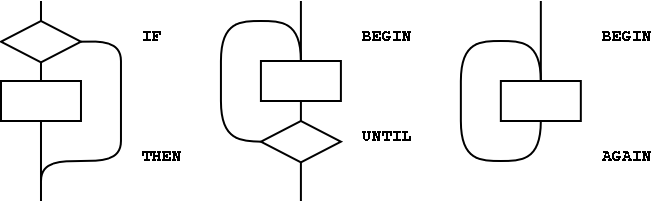
\includegraphics[bb=0 0 658 202,width=0.8\textwidth]{basic.png}}
	\caption{The basic control-flow patterns}
	\label{fig:basic}
  \end{center}
\end{figure}

In control flow every branch, or transfer of control, must terminate
at some destination. A natural implementation uses a stack to
remember the origin of forward branches and the destination of
backward branches. At a minimum, only the location of each origin or
destination must be indicated, although other implementation-dependent
information also may be maintained.

An origin is the location of the branch itself. A destination is
where control would continue if the branch were taken. A destination
is needed to resolve the branch address for each origin, and conversely,
if every control-flow path is completed no unused destinations can
remain.

With the addition of just three words (\word[tools]{AHEAD},
\word[tools]{CS-ROLL} and \word[tools]{CS-PICK}), the basic control-flow
words supply the primitives necessary to compile a variety of transportable
control structures. The abilities required are compilation of forward
and backward conditional and unconditional branches and compile-time
management of branch origins and destinations.
Table~\textbf{\ref{table:control}} shows the desired behavior.

\begin{table}[ht]
  \begin{center}
	\caption{Compilation behavior of control-flow words}
	\label{table:control}
	\begin{tabular}{lccl}
	\hline\hline
	\multicolumn{4}{l}{at compile-time,} \\
	word: & supplies: & resolves: & is used to: \\ \hline
	\word{IF}				& \emph{orig}	&				&	mark origin of forward conditional branch \\
	\word{THEN}			&				& \emph{orig}	&	resolve \word{IF} or \word[tools]{AHEAD} \\
	\word{BEGIN}			& \emph{dest}	&				&	mark backward destination \\
	\word{AGAIN}			&				& \emph{dest}	&	resolve with backward unconditional branch \\
	\word{UNTIL}			&				& \emph{dest}	&	resolve with backward conditional branch \\
	\word[tools]{AHEAD}		& \emph{orig}	&				&	mark origin of forward unconditional branch \\
	\word[tools]{CS-PICK}	&				&				&	copy item on control-flow stack \\
	\word[tools]{CS-ROLL}	&				&				&	reorder items on control-flow stack \\
	\hline\hline
	\end{tabular}
  \end{center}
\end{table}

The requirement that control-flow words are properly balanced by other
control-flow words makes reasonable the description of a compile-time
implementation-defined \emph{control-flow stack}. There is no
prescription as to how the control-flow stack is implemented, e.g.,
data stack, linked list, special array. Each element of the
control-flow stack mentioned above is the same size.

With these tools, the remaining basic control-structure elements,
shown in figure~\textbf{\ref{fig:additional}}, can be defined. The
stack notation used here for immediate words is ( \emph{compilation
/ execution} ).

\begin{quote}\ttfamily
  \begin{tabbing}
	\tab \= \hspace{10em} \= \kill
	\+ \word{:} \word{WHILE}~ \word{p} dest -{}- orig dest / flag -{}- ) \\
		\word{bs} conditional exit from loops \\
		\word{POSTPONE} \word{IF}		\> \word{bs} conditional forward brach \\
	\-	1 \word[tools]{CS-ROLL}			\> \word{bs} keep dest on top \\
	\word{;} \word{IMMEDIATE} \\[2\parskip]

	\+	\word{:} \word{REPEAT}~ \word{p} orig dest -{}- / -{}- ) \\
		\word{bs} resolve a single WHILE and return to BEGIN \\
		\word{POSTPONE} \word{AGAIN}	\> \word{bs} uncond. backward branch to dest \\
	\-	\word{POSTPONE} \word{THEN}		\> \word{bs} resolve forward branch from orig \\
	\word{;} \word{IMMEDIATE} \\[2\parskip]

	\+ \word{:} \word{ELSE}~ \word{p} orig1 -{}- orig2 / -{}- ) \\
		\word{bs} resolve IF supplying alternate execution \\
		\word{POSTPONE} \word[tools]{AHEAD}	\> \word{bs} unconditional forward branch orig2 \\
		1 \word[tools]{CS-ROLL}				\> \word{bs} put orig1 back on top \\
	\-	\word{POSTPONE} \word{THEN}			\> \word{bs} resolve forward branch from orig1 \\
	\word{;} \word{IMMEDIATE}
  \end{tabbing}
\end{quote}

\begin{figure}[ht]
  \begin{center}
	\fbox{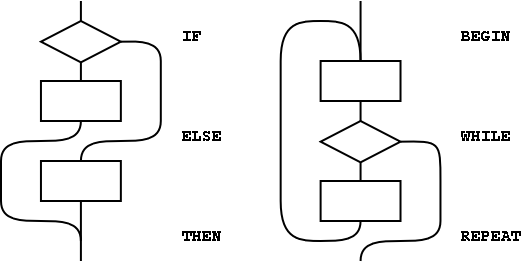
\includegraphics[bb=0 0 529 262,width=0.8\textwidth]{additional.png}}
	\caption{Additional basic control-flow patterns}
	\label{fig:additional}
  \end{center}
\end{figure}

Forth control flow provides a solution for well-known problems with
strictly structured programming.

The basic control structures can be supplemented, as shown in the
examples in figure~\textbf{\ref{fig:extended}}, with additional
\word{WHILE}s in \word{BEGIN} {\ldots} \word{UNTIL} and \word{BEGIN}
{\ldots} \word{WHILE} {\ldots} \word{REPEAT} structures. However, for
each additional \word{WHILE} there must be a \word{THEN} at the end
of the structure. \word{THEN} completes the syntax with \word{WHILE}
and indicates where to continue execution when the \word{WHILE}
transfers control. The use of more than one additional \word{WHILE}
is possible but not common. Note that if the user finds this use of
\word{THEN} undesirable, an alias with a more likable name could be
defined.

Additional actions may be performed between the control flow word (the
\word{REPEAT} or \word{UNTIL}) and the \word{THEN} that matches the
additional \word{WHILE}. Further, if additional actions are desired
for normal termination and early termination, the alternative actions
may be separated by the ordinary Forth \word{ELSE}. The termination
actions are all specified after the body of the loop.

\begin{figure}[ht]
  \begin{center}
	\fbox{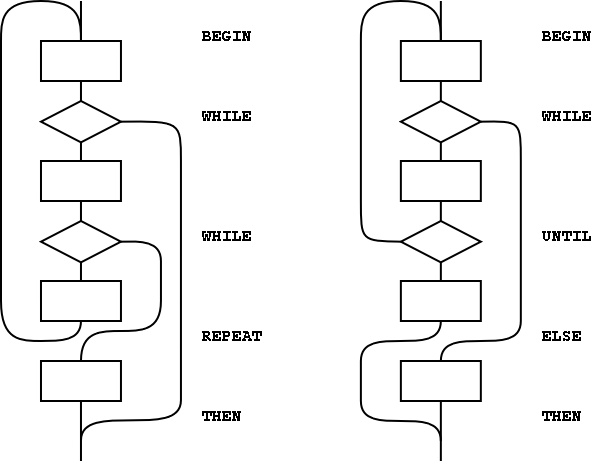
\includegraphics[bb=0 0 598 462, width=0.8\textwidth]{extended.png}}
	\caption{Extended control-flow patterns}
	\label{fig:extended}
  \end{center}
\end{figure}

Note that \word{REPEAT} creates an anomaly when matching the
\word{WHILE} with \word{ELSE} or \word{THEN}, most notably when
compared with the \word{BEGIN}{\ldots}\word{UNTIL} case. That is,
there will be one less \word{ELSE} or \word{THEN} than there are
\texttt{WHILE}s because \word{REPEAT} resolves one \word{THEN}. As
above, if the user finds this count mismatch undesirable, \word{REPEAT}
could be replaced in-line by its own definition.

Other loop-exit control-flow words, and even other loops, can be
defined. The only requirements are that the control-flow stack is
properly maintained and manipulated.

The simple implementation of the \word{CASE} structure
below is an example of control structure extension. Note the
maintenance of the data stack to prevent interference with the
possible control-flow stack usage.

\begin{quote}\ttfamily
  \begin{tabbing}
	\tab \= \hspace{10em} \= \kill
	0 \word{CONSTANT} \word{CASE} \word{IMMEDIATE}~ \word{p} init count of OFs ) \\[2\parskip]

	\+ \word{:} \word{OF}~ \word{p} \#of -{}- orig \#of+1 / x -{}- ) \\
		\word{1+}					\> \word{p} count OFs ) \\
		\word{toR}					\> \word{p} move off the stack in case the control-flow ) \\
									\> \word{p} stack is the data stack. ) \\
		\word{POSTPONE} \word{OVER}~ \word{POSTPONE} \word{=}~
								\word{p} copy and test case value) \\
		\word{POSTPONE} \word{IF}	\> \word{p} add orig to control flow stack ) \\
		\word{POSTPONE} \word{DROP}	\> \word{p} discards case value if = ) \\
	\-	\word{Rfrom}				\> \word{p} we can bring count back now ) \\
	\word{;} \word{IMMEDIATE} \\[2\parskip]

	\+ \word{:} \word{ENDOF}~ \word{p} orig1 \#of -{}- orig2 \#of ) \\
		\word{toR}					\> \word{p} move off the stack in case the control-flow ) \\
									\> \word{p} stack is the data stack. ) \\
		\word{POSTPONE} \word{ELSE} \\
	\-	\word{Rfrom}				\> \word{p} we can bring count back now ) \\
	\word{;} \word{IMMEDIATE} \\[2\parskip]

	\+ \word{:} \word{ENDCASE}~ \word{p} orig1..orign \#of -{}- ) \\
		\word{POSTPONE} \word{DROP}	\> \word{p} discard case value ) \\
		0 \word{qDO} \\
		\tab \word{POSTPONE} \word{THEN} \\
	\- \word{LOOP} \\
	\word{;} \word{IMMEDIATE}
  \end{tabbing}
\end{quote}

\paragraph{Return stack} ~ % A.3.2.3.3

The restrictions in section \xref[3.2.3.3 Return stack]{usage:returnstack}
are necessary if implementations are to be allowed to place loop
parameters on the return stack.

\addtocounter{subsubsection}{2}
\subsubsection{Environmental queries} % A.3.2.6

The size in address units of various data types may be determined by
phrases such as \texttt{1} \word{CHARS}. Similarly, alignment may be
determined by phrases such as \texttt{1} \word{ALIGNED}.

The environmental queries are divided into two groups: those that
always produce the same value and those that might not. The former
groups include entries such as \texttt{MAX-N}. This information is
fixed by the hardware or by the design of the Forth system; a user
is guaranteed that asking the question once is sufficient.

The other, now obsolescent, group of queries are for things that may
legitimately change over time. For example an application might test
for the presence of the Double Number word set using an environment
query.  If it is missing, the system could invoke a system-dependent
process to load the word set. The system is permitted to change
\word{ENVIRONMENTq}'s database so that subsequent queries about
it indicate that it is present.

Note that a query that returns an ``unknown'' response could produce
a ``known'' result on a subsequent query.

\subsubsection{Obsolescent Environmental Queries} % A.3.2.7
\label{rat:obsolete}

When reviewing the Forth 94 Standard, the question of adapting the
word set queries had to be addressed.  Despite the recommendation
in Forth 94, word set queries have not been
supported in a meaningful way by many systems.  Consequently, these
queries are not used by many programmers.  The committee was unwilling
to exacerbate the problem by introducing additional queries for the
revised word sets.  The committee has therefore declared the word set
environment queries (see table \ref{table:obsolete}) as obsolescent
with the intention of removing them altogether in the next revision.
They are retained in this standard to support existing Forth 94
programs.  New programs should not use them.

\subsubsection{Extension queries} % A.3.2.8

\subsection{The Forth dictionary} % A.3.3

A Standard Program may redefine a standard word with a non-standard
definition. The program is still standard (since it can be built on
any Standard System), but the effect is to make the combined entity
(Standard System plus Standard Program) a non-standard system.

\subsubsection{Name space} % A.3.3.1

\setcounter{paragraph}{1}
\paragraph{Definition names} ~ % A.3.3.1.2

The language in this section is there to ensure the portability of
Standard Programs. If a program uses something outside the Standard
that it does not provide itself, there is no guarantee that another
implementation will have what the program needs to run. There is no
intent whatsoever to imply that all Forth programs will be somehow
lacking or inferior because they are not standard; some of the finest
jewels of the programmer's art will be non-standard. At the same time,
the committee is trying to ensure that a program labeled ``Standard''
will meet certain expectations, particularly with regard to portability.

In many system environments the input source is unable to supply
certain non-graphic characters due to external factors, such as the
use of those characters for flow control or editing. In addition,
when interpreting from a text file, the parsing function specifically
treats non-graphic characters like spaces; thus words received by the
text interpreter will not contain embedded non-graphic characters. To
allow implementations in such environments to call themselves standard,
this minor restriction on Standard Programs is necessary.

A Standard System is allowed to permit the creation of definition
names containing non-graphic characters. Historically, such names
were used for keyboard editing functions and ``invisible'' words.

\subsubsection{Code space} % A.3.3.2

\subsubsection{Data space} % A.3.3.3
\label{rat:dataspace}

The words \word{toIN}, \word{BASE}, \word[block]{BLK}, \word[block]{SCR},
\word{SOURCE}, \word{SOURCE-ID}, \word{STATE}  contain information
used by the Forth system in its operation and may be of use to the
application. Any assumption made by the application about data
available in the Forth system it did not store other than the data
just listed is an environmental dependency.

There is no point in specifying (in the Standard) both what is and
what is not addressable. A Standard Program may NOT address:

\begin{itemize}
\item Directly into the data or return stacks;
\item Into a definition's data field if not stored by the application.
\end{itemize}

The read-only restrictions arise because some Forth systems run from
ROM and some share I/O buffers with other users or systems. Portable
programs cannot know which areas are affected, hence the general
restrictions.

\paragraph{Address alignment} ~ % A.3.3.3.1
\label{rat:aaddr}

Some processors have restrictions on the addresses that can be used
by memory access instructions. For example, some architectures require
16-bit data to be loaded or stored only at even addresses and 32-bit
data only at addresses that are multiples of four.

An implementor can handle these alignment restrictions in one of two
ways. Forth's memory access words (\word{@}, \word{!}, \word{+!},
etc.) could be implemented in terms of smaller-width access instructions,
which have no alignment restrictions.  For example, on a system with
16-bit cells, \word{@} could be implemented with two byte-fetch
instructions and a reassembly of the bytes into a 16-bit cell.  Although
this conceals hardware restrictions from the programmer, it is inefficient,
and may have unintended side effects in some hardware environments.
An alternate implementation could define each memory-access word
using the native instructions that most closely match the word's function.
The 16-bit cell system could implement \word{@} using the processor's
16-bit fetch instruction, in this case, the responsibility for giving
\word{@} a correctly-aligned address falls on the programmer.  A
portable program must assume that alignment may be required and
follow the requirements of this section.

\newpage
\paragraph{Contiguous regions} ~ % A.3.3.3.2
\label{rat:regions}

The data space of a Forth system comes in discontiguous regions. The
location of some regions is provided by the system, some by the
program. Data space is contiguous within regions, allowing address
arithmetic to generate valid addresses only within a single region.
A Standard Program cannot make any assumptions about the relative
placement of multiple regions in memory.

Section \ref{usage:contiguous} does prescribe conditions under which
contiguous regions of data space may be obtained. For example:
\begin{quote}\ttfamily
	\word{CREATE} TABLE \quad
	1 \word{C,} 2 \word{C,} \word{ALIGN} 1000 \word{,} 2000 \word{,}
\end{quote}
makes a table whose address is returned by \texttt{TABLE}. In
accessing this table,
\begin{quote}
  \begin{tabular}{ll}
	\texttt{TABLE} \word{C@}					& will return 1 \\
	\texttt{TABLE} \word{CHAR+} \word{C@}		& will return 2 \\
	\texttt{TABLE} \texttt{2} \word{CHARS} \word{+}
		\word{ALIGNED} \word{@}					& will return 1000 \\
	\texttt{TABLE} \texttt{2} \word{CHARS} \word{+}
		\word{ALIGNED} \word{CELL+} \word{@}	&  will return 2000. \\
  \end{tabular}
\end{quote}
Similarly,
\begin{quote}\ttfamily
	\word{CREATE} DATA \quad 1000 \word{ALLOT}
\end{quote}
makes an array 1000 address units in size. A more portable strategy
would define the array in application units, such as:
\begin{quote}\ttfamily
	500 \word{CONSTANT} NCELLS \\
	\word{CREATE} CELL-DATA NCELLS \word{CELLS} \word{ALLOT}
\end{quote}

This array can be indexed like this:
\begin{quote}\ttfamily
	\word{:} LOOK \quad
		NCELLS 0 \word{DO}
			CELL-DATA \word{I} \word{CELLS} \word{+} \word[tools]{q}
		\word{LOOP}
	\word{;}
\end{quote}


\setcounter{paragraph}{5}
\paragraph{Other transient regions} ~ % A.3.3.3.6

In many existing Forth systems, these areas are at \word{HERE} or
just beyond it, hence the many restrictions.

$(2*n)+2$ is the size of a character string containing the
unpunctuated binary representation of the maximum double number with
a leading minus sign and a trailing space.

Implementation note: Since the minimum value of \param{n} is 16, the
absolute minimum size of the pictured numeric output string is 34
characters. But if your implementation has a larger \param{n}, you must
also increase the size of the pictured numeric output string.

\subsection{The Forth text interpreter} % A.3.4

\setcounter{subsubsection}{2}
\subsubsection{Semantics} % A.3.4.3

The ``initiation semantics'' correspond to the code that is executed
upon entering a definition, analogous to the code executed by
\word{EXIT} upon leaving a definition. The ``run-time semantics''
correspond to code fragments, such as literals or branches, that are
compiled inside colon definitions by words with explicit compilation
semantics.

In a Forth cross compiler, the execution semantics may be specified
to occur in the host system only, the target system only, or in both
systems. For example, it may be appropriate for words such as
\word{CELLS} to execute on the host system returning a value describing
the target, for colon definitions to execute only on the target, and
for \word{CONSTANT} and \word{VARIABLE} to have execution behaviors on
both systems. Details of cross compiler behavior are beyond the scope
of this standard.

\setcounter{paragraph}{1}
\paragraph{Interpretation semantics} ~ % A.3.4.3.2
\label{rat:interpret}

For a variety of reasons, this standard does not define interpretation
semantics for every word. Examples of these words are \word{toR},
\word{.q}, \word{DO}, and \word{IF}. Nothing in this Standard precludes
an implementation from providing interpretation semantics for these
words, such as interactive control-flow words. However, a Standard
Program may not use them in interpretation state.

\addtocounter{subsubsection}{1}
\subsubsection{Compilation} % A.3.4.5

Compiler recursion at the definition level consumes excessive
resources, especially to support locals. The committee does not
believe that the benefits justify the costs. Nesting definitions
is also not common practice and won't work on many systems.

\section{Documentation requirements} % A.4 ==========================

\subsection{System documentation} % A.4.1

\subsection{Program documentation} % A.4.2

\section{Compliance and labeling} % A.5 =============================

\subsection{Forth-\snapshot{} systms} % A.5.1

Section \ref{label:label} defines the criteria that a system must
meet in order to justify the label ``Forth-\snapshot{} System''. Briefly,
the minimum requirement is that the system must ``implement'' the
Core word set. There are several ways in which this requirement may
be met. The most obvious is that all Core words may be in a pre-compiled
kernel. This is not the only way of satisfying the requirement,
however. For example, some words may be provided in source blocks or
files with instructions explaining how to add them to the system if
they are needed. So long as the words are provided in such a way that
the user can obtain access to them with a clear and straightforward
procedure, they may be considered to be present.

A Forth cross compiler has many characteristics in common with a standard
system, in that both use similar compiling tools to process a program.
However, in order to fully specify a Forth-\snapshot{} standard
cross compiler it would be necessary to address complex issues dealing with
compilation
and execution semantics in both host and target environments as well as
ROMability issues. The level of effort to do this properly has proved to
be impractical at this time. As a result, although it may be possible
for a Forth cross compiler to correctly prepare a Forth-\snapshot{}
standard program for execution in a target environment, it is inappropriate
for a cross compiler to be labeled a Forth-\snapshot{} standard system.

\subsection{Forth-\snapshot{} programs} % A.5.2

\setcounter{subsubsection}{1}
\subsubsection{Program labeling} % A.5.2.2

Declaring an environmental dependency should not be considered
undesirable, merely an acknowledgment that the author has taken
advantage of some assumed architecture. For example, most computers
in common use are based on two's complement binary arithmetic. By
acknowledging an environmental dependency on this architecture,
a programmer becomes entitled to use the number \texttt{-1} to
represent all bits set without significantly restricting the
portability of the program.

Because all programs require space for data and instructions, and
time to execute those instructions, they depend on the presence of
an environment providing those resources. It is impossible to predict
how little of some of these resources (e.g. stack space) might be
necessary to perform some task, so this standard does not do so.

On the other hand, as a program requires increasing levels of
resources, there will probably be sucessively fewer systems on
which it will execute sucessfully. An algorithm requiring an array
of $10^9$ cells might run on fewer computers than one requiring
only $10^3$.

Since there is also no way of knowing what minimum level of resources
will be implemented in a system useful for at least some tasks, any
program performing real work labeled simply
a ``Standard Forth-\snapshot{} Program'' is unlikely to be labeled
correctly.


\section{Glossary} % A.6 ============================================

In this and following sections we present rationales for the handling
of specific words: why we included them, why we placed them in certain
word sets, or why we specified their names or meaning as we did.

Words in this section are organized by word set, retaining their index
numbers for easy cross-referencing to the glossary.

Historically, many Forth systems have been written in Forth. Many of
the words in Forth originally had as their primary purpose support of
the Forth system itself. For example, \word{WORD} and \word{FIND} are
often used as the principle instruments of the Forth text interpreter,
and \word{CREATE} in many systems is the primitive for building
dictionary entries. In defining words such as these in a standard way,
we have endeavored not to do so in such a way as to preclude their use
by implementors. One of the features of Forth that has endeared it to
its users is that the same tools that are used to implement the system
are available to the application programmer --- a result of this
approach is the compactness and efficiency that characterizes most
Forth implementations.

\readrationale{core}

\setcounter{subsection}{1}
\subsection{Core extension words} % A.6.2 =================
\label{rat:core-ext}

The words in this collection fall into several categories:

\begin{itemize}
\item Words that are in common use but are deemed less essential than
	Core words (e.g., \word{0ne});

\item Words that are in common use but can be trivially defined from
	Core words (e.g., \word{FALSE});

\item Words that are primarily useful in narrowly defined types of
	applications or are in less frequent use (e.g., \word{PARSE});

\item Words that are being deprecated in favor of new words introduced
	to solve specific problems.
\end{itemize}

Because of the varied justifications for inclusion of these words,
the committee does not encourage implementors to offer the complete
collection, but to select those words deemed most valuable to their
clientele.

\readrationale{core-ext}


\section{The optional Block word set} % A.7 =========================
\setwordlist{block}
\label{rat:block}

Early Forth systems ran without a host OS; these are known as native
systems.  Such systems provide mass storage in blocks of 1024 bytes.
The Block Word set includes the most common words for accessing
program source and data on disk.

\setcounter{subsection}{1}
\subsection{Additional terms} % A.7.2 ===============================
\label{rat:block:terms}

\begin{description}
\item[block] ~

	Forth systems may use blocks to contain program source.
	Conventionally such blocks are formatted for editing as
	16 lines of 64 characters. Source blocks are often referred
	to as ``screens''.
\end{description}

\subsection{Additional usage requirements}
\setcounter{subsubsection}{1}
\subsubsection{Block buffer regions}
\label{rat:block:buffers}

	While the standard does not address multitasking per se, the
	items listed in \xref{block:buffers} that may render block-buffer
	addresses invalid are due to multitasking considerations.
	The standard restricts programs such that items that could fail on
	multitasking systems are not standard usage.  It also permits
	multitasking systems to be declared standard systems.

\setcounter{subsection}{5}
\subsection{Glossary} % A.7.6 =============================

\readrationale{block}


\section{The optional Double-Number word set} % A.8 =================
\setwordlist{double}
\label{rat:double}

Forth systems on 8-bit and 16-bit processors often find it necessary
to deal with double-length numbers. But many Forths on small embedded
systems do not, and many users of Forth on systems with a cell size of
32-bits or more find that the necessity for double-length numbers is
much diminished. Therefore, we have factored the words that manipulate
double-length entities into this optional word set.

Please note that the naming convention used in this word set conveys
some important information:

\begin{enumerate}
\item[1.]
	Words whose names are of the form \texttt{2}\emph{xxx} deal
	with cell pairs, where the relationship between the cells is
	unspecified. They may be two-vectors, double-length numbers, or
	any pair of cells that it is convenient to manipulate together.

\item[2.]
	Words with names of the form \texttt{D}\emph{xxx} deal
	specifically with double-length integers.

\item[3.]
	Words with names of the form \texttt{M}\emph{xxx} deal with
	some combination of single and double integers. The order in
	which these appear on the stack is determined by long-standing
	common practice.
\end{enumerate}

Refer to \ref{rat:types} for a discussion of data types in Forth.

\setcounter{subsection}{5}
\subsection{Glossary} % A.8.6 =============================

\readrationale{double}


\section{The optional Exception word set} % A.9 =====================
\setwordlist{exception}
\label{rat:exception}

\word{CATCH} and \word{THROW} provide a reliable mechanism for
handling exceptions, without having to propagate exception flags
through multiple levels of word nesting. It is similar in spirit
to the ``non-local return'' mechanisms of many other languages,
such as C's \texttt{setjmp()} and \texttt{longjmp()}, and LISP's
\texttt{CATCH} and \texttt{THROW}. In the Forth context, \word{THROW}
may be described as a ``multi-level \word[core]{EXIT}'', with
\word{CATCH} marking a location to which a \word{THROW} may return.

Several similar Forth ``multi-level \word[core]{EXIT}''
exception-handling schemes have been described and used in past years.
It is not possible to implement such a scheme using only standard words
(other than \word{CATCH} and \word{THROW}), because there is no portable
way to ``unwind'' the return stack to a predetermined place.

\word{THROW} also provides a convenient implementation technique for
the standard words \word{ABORT} and \word{ABORTq}, allowing an
application to define, through the use of \word{CATCH}, the behavior
in the event of a system \word{ABORT}.

\word{CATCH} and \word{THROW} provide a convenient way for an
implementation to ``clean up'' the state of open files if an
exception occurs during the text interpretation of a file with
\word[file]{INCLUDE-FILE}. The implementation of
\word[file]{INCLUDE-FILE} may guard (with \word{CATCH}) the word
that performs the text interpretation, and if \word{CATCH} returns
an exception code, the file may be closed and the exception
re\word{THROW}n so that the files being included at an outer nesting
level may be closed also. Note that the standard allows, but does not
require, \word[file]{INCLUDE-FILE} to close its open files if an
exception occurs. However, it does require \word[file]{INCLUDE-FILE}
to unnest the input source specification if an exception is
\word{THROW}n.

\setcounter{subsection}{2}
\subsection{Additional usage requirements} % A.9.3 ========

One important use of an exception handler is to maintain program
control under many conditions which \word{ABORT}.  This is practicable
only if a range of codes is reserved.  Note that an application may
overload many standard words in such a way as to \word{THROW}
ambiguous conditions not normally \word{THROW}n by a particular
system.

\setcounter{subsubsection}{5}
\subsubsection{Exception handling} % A.9.3.6 ==============

The method of accomplishing this coupling is implementation dependent.
For example, \word[block]{LOAD} could ``know'' about \word{CATCH} and
\word{THROW} (by using \word{CATCH} itself, for example), or
\word{CATCH} and \word{THROW} could ``know'' about \word[block]{LOAD}
(by maintaining input source nesting information in a data structure
known to \word{THROW}, for example). Under these circumstances it is
not possible for a Standard Program to define words such as
\word[block]{LOAD} in a completely portable way.

\setcounter{subsection}{5}
\subsection{Glossary} % A.9.6 =============================

\readrationale{exception}


\section{The optional Facility word set} % A.10 =====================
\setwordlist{facility}
\label{rat:facility}

\setcounter{subsection}{5}
\subsection{Glossary} % A.10.6 ============================

\readrationale{facility}


\section{The optional File-Access word set} % A.11 ==================
\setwordlist{file}
\label{rat:file}

\setcounter{subsection}{2}
\subsection{Additional usage requirements} % A.11.3 =======

\setcounter{subsubsection}{1}
\subsubsection{Blocks in files} % 11.3.2 ==================

Many systems reuse file identifiers; when a file is closed, a
subsequently opened file may be given the same identifier. If the
original file has blocks still in block buffers, these will be
incorrectly associated with the newly opened file with disastrous
results. The block buffer system must be flushed to avoid this.

\setcounter{subsubsection}{3}
\subsubsection{Other transient regions}
\label{rat:file:buffers}

Additional transient buffers are provided for use by \word{Sq} and \word{Seq}.
The buffers should be able to store two consecutive strings, thus allowing the
command line:

\begin{quote}
	\texttt{\word{Sq} name1" \word{Sq} name2" \word{RENAME-FILE}}
\end{quote}

The buffers may be implemented in a circular arrangement, where a string
is placed into the next available buffer. When there are no buffers available,
the oldest buffer is overwritten.

\word{Sq} and \word{Seq} may share the same buffers.

The list of words using memory in transient regions is extended to include
\wref{file:Sq}{} and \wref{file:Seq}{}.
See \xref[3.3.3.6 Other transient regions]{usage:transient}.

\setcounter{subsection}{5}
\subsection{Glossary} % A.11.6 ============================

\readrationale{file}


\section{The optional Floating-Point word set} % A.12 ===============
\setwordlist{floating}
\label{rat:floating}

	The current base for floating-point input must be \word{DECIMAL}.
	Floating-point input is not allowed in an arbitrary base. All
	floating-point numbers to
	be interpreted by a standard system must contain the exponent
	indicator ``\texttt{E}'' (see \xref[12.3.7 Text	interpreter input
	number conversion]{float:conv}). Consensus in the committee deemed
	this form of floating-point input to be in more common use than
	the alternative that would have a floating-point input mode that
	would allow numbers with embedded decimal points to be treated
	as floating-point numbers.

	Although the format and precision of the significand and the format
	and range of the exponent of a floating-point number are
	implementation defined in Forth-\snapshot, the Floating-Point
	Extensions word set contains the words
	\word{DF@}, \word{SF@}, \word{DF!}, and \word{SF!}
	for fetching and storing double- and single-precision IEEE
	floating-point-format numbers to memory. The IEEE floating-point
	format is commonly used by numeric math co-processors and for
	exchange of floating-point data between programs and systems.

\setcounter{subsection}{2}
\subsection{Additional usage requirements} % A.12.3 =======

\setcounter{subsubsection}{4}
\subsubsection{Address alignment} % A.12.3.5 ==============

In defining custom floating-point data structures, be aware that
\word{CREATE} doesn't necessarily leave the data space pointer
aligned for various floating-point data types. Programs may comply
with the requirement for the various kinds of floating-point alignment
by specifying the appropriate alignment both at compile-time and
execution time. For example:

\begin{quote}\ttfamily
	\word{:} \word{FCONSTANT} \word{p} F: r -{}- ) \\
	\tab \word{CREATE} \word{FALIGN} ~\word{HERE}~
		1 \word{FLOATS} \word{ALLOT} ~\word{F!} \\
	\tab \word{DOES} \word{p} F: -{}- r )
		~\word{FALIGNED} \word{F@} \word{;}
\end{quote}

\setcounter{subsubsection}{6}
\subsubsection{Text interpreter input number conversion} % A.12.3.7

The committee has more than once received the suggestion that the
text interpreter in standard Forth systems should treat numbers
that have an embedded decimal point, but no exponent, as
floating-point numbers rather than double cell numbers. This
suggestion, although it has merit, has always been voted down because
it would break too much existing code; many existing implementations
put the full digit string on the stack as a double number and use
other means to inform the application of the location of the decimal
point.

\setcounter{subsection}{5}
\subsection{Glossary} % A.12.6 ============================

\readrationale{floating}


\section{The optional Locals word set} % A.13 =======================
\setwordlist{local}
\label{rat:local}

\setcounter{subsection}{2}
\subsection{Additional usage requirements} % A.13.3 =======

Rule \ref{locals:rules}d could be relaxed without affecting the
integrity of the rest of this structure. \ref{locals:rules}c could
not be.

\ref{locals:rules}b forbids the use of the data stack for local
storage because no usage rules have been articulated for programmer
users in such a case. Of course, if the data stack is somehow employed
in such a way that there are no usage rules, then the locals are
invisible to the programmer, are logically not on the stack, and the
implementation conforms.

Access to previously declared local variables is prohibited by Section
\ref{locals:rules}d until any data placed onto the return stack by the
application has been removed, due to the possible use of the return
stack for storage of locals.

Authorization for a Standard Program to manipulate the return stack
(e.g., via \word[core]{toR} \word[core]{Rfrom}) while local variables
are active overly constrains implementation possibilities. The consensus
of users of locals was that Local facilities represent an effective
functional replacement for return stack manipulation, and restriction
of standard usage to only one method was reasonable.

Access to Locals within \word[core]{DO}{\ldots}\word[core]{LOOP}s is
expressly permitted as an additional requirement of conforming systems
by Section \ref{locals:rules}g. Although words, such as \word{LOCAL},
written by a System Implementor, may require inside knowledge of the
internal structure of the return stack, such knowledge is not required
of a user of compliant Forth systems.

\setcounter{subsection}{5}
\subsection{Glossary} % A.13.6 ============================

\readrationale{local}


\section{The optional Memory-Allocation word set} % A.14 ============
\setwordlist{memory}
\label{rat:memory}

The Memory-Allocation word set provides a means for acquiring memory
other than the contiguous data space that is allocated by \word{ALLOT}.
In many operating system environments it is inappropriate for a process
to pre-allocate large amounts of contiguous memory (as would be
necessary for the use of \word{ALLOT}).  The Memory-Allocation word set
can acquire memory from the system at any time, without knowing in
advance the address of the memory that will be acquired.


\section{The optional Programming-Tools word set} % A.15 ============
\setwordlist{tools}
\label{rat:tools}

These words have been in widespread common use since the earliest
Forth systems.

Although there are environmental dependencies intrinsic to programs
using an assembler, virtually all Forth systems provide such a
capability. Insofar as many Forth programs are intended for real-time
applications and are intrinsically non-portable for this reason, the
committee believes that providing a standard window into
assemblers is a useful contribution to Forth programmers.

Similarly, the programming aids \word{DUMP}, etc., are valuable tools
even though their specific formats will differ between CPUs and Forth
implementations. These words are primarily intended for use by the
programmer, and are rarely invoked in programs.

One of the original aims of Forth was to erase the boundary between
``user'' and ``programmer'' --- to give all possible power to anyone
who had occasion to use a computer. Nothing in the above labeling or
remarks should be construed to mean that this goal has been abandoned.

\setcounter{subsection}{3}
\subsubsection{Name tokens}
\label{rat:tools:nt}

Name tokens are an abstract data type identifying named words.
You can use words such as \word{NAMEtoSTRING} to get information
out of name tokens.


\setcounter{subsection}{5}
\subsection{Glossary} % A.15.6 ============================

\readrationale{tools}


\section{The optional Search-Order word set} % A.16 =================
\setwordlist{search}
\label{rat:search}

The search-order word set is intended to be a portable ``construction
set'' from which search-order words may be built.  \word{ALSO}/\word{ONLY}
or the various ``vocabulary'' schemes supported by the major Forth
vendors can be defined in terms of the primitive search-order word set.

The encoding for word list identifiers \emph{wid} might be a
small-integer index into an array of word-list definition records, the
data-space address of such a record, a user-area offset, the execution
token of a sealed vocabulary, the link-field address of the first definition
in a word list, or anything else. It is entirely up to the system implementor.

\setcounter{subsection}{1}
\subsection{Additional terms and notation} % A.16.2 =================

\begin{description}
\item[search order] ~

	Note that the use of the term ``list'' does not necessarily
	imply implementation as a linked list
\end{description}

\pagebreak
\subsection{Additional usage requirements} % A 16.3 ============

\setcounter{subsubsection}{2}
\subsubsection{Finding definition names} % A.16.3.3 =======

In other words, the following is not guaranteed to work:

\begin{quote}\ttfamily
	\word{:} FOO {\ldots}
		\word{[} {\ldots} \word{SET-CURRENT} \word{]}
		{\ldots} \word{RECURSE} {\ldots} \\
	\word{;} \word{IMMEDIATE}
\end{quote}
\word{RECURSE}, \word{;} (semicolon), and \word{IMMEDIATE} may
or may not need information stored in the compilation word list.

\setcounter{subsection}{5}
\subsection{Glossary} % A.16.6 ============================

\readrationale{search}

\section{The optional String word set} % A.17 =======================
\setwordlist{string}
\label{rat:string}


\setcounter{subsection}{5}
\subsection{Glossary} % A.17.6 ============================

\readrationale{string}


\section{The optional Extended-Character word set} % A.18 =======================
\setwordlist{xchar}
\label{rat:xchar}

Forth defines graphic and control characters from the ASCII character
set.  ASCII was originally designed for the English language.
However, most western languages fit somewhat into the Forth framework,
since a single byte is sufficient to encode all characters in each
language, although different languages may use different encodings;
Latin-1 and Latin-15 are widely used.  For other languages, different
character sets have to be used, several of which are variable-width.
Currently, the most popular representative of the variable-width
character sets is UTF-8.

Many Forth systems today are case insensitive, to accept lower case
standard words.  It is sufficient to be case insensitive for the ASCII
subset to make this work --- this saves a large code mapping table for
comparison of other symbols.  Case is mostly an issue of European
languages (Latin, Greek, and Cyrillic), but similar issues exist
between traditional and simplified Chinese (finally being dealt with
by Unihan), and between different Latin code pages in the Universal
Character Set (UCS), e.g., full width vs.\ normal half width Latin
letters.

Furthermore, UCS allows composition of glyphs and has direct encoding for
composed glyphs, which look the same, but have different encodings.  This
is not a problem for a Forth system to solve.

Some encodings (not UTF-8) might give surprises when you use a case
insensitive ASCII-compare that's 8-bit safe, but not aware of the
current encoding.

The xchar word set does not address problems that come from using
multiple different encodings and switching or converting between them.
It is good practice for a system implementing xchar to support UTF--8.

\setcounter{subsection}{5}
\subsection{Glossary} % A.18.6 ============================

\readrationale{xchar}

\endinput
